\chapterimage{chapter_head_teclado.pdf} % Chapter heading image

\chapter{Fundamentos de notação musical}
Nas seguintes sub seções abordaremos alguns conceitos de notação musical;
porem, não aprofundaremos demasiado em toda a teoria musical, 
devido a que as explicações mostradas aqui, estão
orientadas para um público interessado na dança, que numa primeira 
aproximação à música, precisa conhecer rapidamente conceitos básicos. 
Mas, empoderamos a curiosidade de todos os leitores a aprofundar mais nestos temas, 
para este efeito existem na literatura muitos materiais, livros ou revistas especializadas 
\cite{medteoria}        %% Teoria Da Musica
\cite{cardoso1973curso} %% Curso Completo De Teoria Musical E Solfejo - 1o Vol.
\cite{mascarenhascurso} %% Curso Completo De Teoria Musical E Solfejo - 2o Vol.
\cite{grabner2001teoria}%% Teoría general de la música 
\cite{alves2004teoria}  %% teoria musical lições essenciais
\cite{apel1969harvard}  %% harvard diccionario
\cite{azevedocompor}    %% Como Compor Música Facilmente: métodos ou estudos para teoria, canto e solfejo (NOPDF)
\cite{adolfo2002musica}.%% Musica: Leitura, Conceitos, Exercicios (NOPDF)

%%%%%%%%%%%%%%%%%%%%%%%%%%%%%%%%%%%%%%%%%%%%%%%%%%%%%%%%%%%%%%%%%%%%%%%%%%%%%%%%

%%%%%%%%%%%%%%%%%%%%%%%%%%%%%%%%%%%%%%%%%%%%%%%%%%%%%%%%%%%%%%%%%%%%%%%%%%%%%%%%
\section{Componentes da música}

A música; na sua forma mais básica,  é um conjunto de sons; esta é criada ao combinar na justa medida: 
ingênio, técnica e arte.

Entre as características de um som temos \cite[pp. 12]{medteoria} :
\begin{description}
\item [Altura:] \label{sec:pos:Altura} 
Também chamado \textbf{tom}\footnote{A palavra tom tem vários significados em música, 
outro significado pode ser um intervalo ou distancia em frequência, 
utilizado na escala diatônica, para mais detalhes ir a Seção \ref{sec:notasmusicais}}, representa a frequência de vibração (principal) da onda mecânica que gera o sonido.
Isto é, que terão um altura maior os sonidos com maior frequência de vibração mecânica (mais agudos), 
e uma altura menor sonidos mais graves.
\begin{example}
A campainha pra chamar ao atendente de um hotel tem uma altura maior,
que a campana da igreja, que é tocada ao médio dia, que tem um sonido mais grave.
\end{example} 
\index{Altura}\index{Tom}
\item [Duração:] \label{sec:pos:Duracion}
Representa a longitude temporal, durante o qual um sonido será executado.
\begin{example}
Podemos assoviar durante um tempo, curto, longo, muito longo, etc.
\end{example} 
\index{Duração}
\item [Intensidade:] \label{sec:pos:Intensidade}
Se refere ao volume sonoro ou à potencia do sonido executado, 
de modo que o som pode ter intensidades, por exemplo: fracas, fortes, muito fortes, etc.  
\begin{example}
Si escolhemos dois pedaços de madeira e batimos eles um contra outro, 
podemos gerar sons com diferente intensidade, dependendo da força com que realizemos os batimentos.
\end{example} 
\index{Intensidade}
\item [Timbre:] \label{sec:pos:timbre}
Na definição da altura de um som, referenciamos esta seguindo a sua frequência principal,
porem um som não está composto exclusivamente por vibrações a esta frequência.
Na pratica os sons contem muitas outras frequências de vibração, acontecendo simultaneamente e 
que se manifestam com menor intensidade.
A combinação de todas estas frequências de vibração é o que gera o som que escutamos;
assim, a essa especifica configuração de frequências a chamamos como o timbre ou
a ``\textbf{cor}'' do som.
\begin{example}
Se geramos dois sonidos com a mesma altura; mas, um sonido executado por uma flauta,
e o outro por um violão, ambos sonidos terão diferentes timbres ou cores.
\end{example} 
\index{Timbre}
\end{description}
~\\

Conhecidas estas definições básicas, e procurando estruturas mais complexas na música,
podemos distinguir alguns componentes com que esta é constituída, 
por exemplo temos:

\begin{description}
\item [Ritmo:] \label{sec:pos:Ritmo}
Se refere a distribuição temporal da execução dos sonidos e a proporção na duração destes. 
Asim, o ritmo carateriza a música no âmbito temporal \cite[pp. 11]{medteoria}.
\index{Ritmo}
\begin{example}
Batendo palmas, criamos a sequencia de sonidos: palmas, pausa curta, palmas, palmas, pausa loga e palmas.
\end{example} 
\item [Melodia:] \label{sec:pos:Melodia}
É um conjunto de sons, que podem ter diferentes \hyperref[sec:pos:Altura]{\textbf{alturas}}, 
e que estão dispostos sequencialmente. 
A melodia representa um elemento horizontal\footnote{\label{eixohor}Eixo com múltiplas distribuições de tempo dos sons na música} na musica, 
e esta é indivisível do ritmo \cite[pp. 517]{apel1969harvard} \cite[pp. 11]{medteoria}.
\begin{example}
Se assoviamos ``parabéns pra você'', estamos executando uma melodia 
(executando diferentes sons numa distribuição temporal especifica).
\end{example} 
\index{Melodia} 
\item [Harmonia:] \label{sec:pos:Harmonia}
Conjunto de sons dispostos simultaneamente em \hyperref[sec:pos:Altura]{\textbf{alturas}} diferentes.
A harmonia representa um elemento vertical\footnote{\label{eixover}Eixo com múltiplas distribuições de frequência dos sons na música} na música \cite[pp. 371]{apel1969harvard} \cite[pp. 8]{cardoso1973curso} \cite[pp. 11]{medteoria}. 
\begin{example}
Se num piano pressionamos simultaneamente as teclas: Do, Mi e Sol. Estamos executando uma harmonia.
\end{example} 
\index{Harmonia} 
\item [Contraponto:] \label{sec:pos:Contraponto}
O termo deriva de ``punctus contra punctum'' que significa ``nota contra nota'', 
e por extensão ``melodia contra melodia''. 
Assim, falar de contraponto é equivalente a dizer, dois ou mais melodias executadas simultaneamente  
(concepção horizontal\footref{eixohor} e vertical\footref{eixover} da música)  \cite[pp. 208]{apel1969harvard} \cite[pp. 11]{medteoria}.
\begin{example}
Uma orquestra com vários músicos tocando cada um uma melodia.
\end{example} 
\index{Contraponto}
\end{description}


 
%%%%%%%%%%%%%%%%%%%%%%%%%%%%%%%%%%%%%%%%%%%%%%%%%%%%%%%%%%%%%%%%%%%%%%%%%%%%%%%%
\section{Figuras musicais, pausas e durações}
\index{Música!Figuras musicais}
\index{Música!Figuras rítmicas}
\label{sec:figurasmusicais}
As figuras musicais também chamada figuras rítmicas \cite[pp. 16]{alves2004teoria}, 
são um conjunto de sinais (desenhos), criadas pra indicar a relação 
entre as \hyperref[sec:pos:Duracion]{\textbf{durações}} dos sons \cite[pp. 20]{medteoria}.
Assim, podemos ver na coluna dois da Tabela \ref{tab:abc-noteslengthbasic}
 um conjunto de 6 destas figuras musicais; 
a primeira coluna representa a longitude temporal (\hyperref[sec:pos:Duracion]{\textbf{duração}}) de cada uma destas figuras;
porém, todos estas durações são relativas ao valor temporal $S$, em segundos, de uma figura \Ganz.
A terceira coluna da tabela contem os nomes de cada uma destas figuras musicais. 
\begin{table}[h]
\centering
\begin{tabular}{|c||c|c||c|c|}
\hline
Duração & Figura & Nome de figura & Pausa & Nome de pausa\\ \hline
\hline
$S$    & \Ganz   & Semibreve    & \GaPa  & Pausa de Semibreve \\ \hline
$S/2$  & \Halb   & Mínima       & \HaPa  & Pausa de Mínima \\ \hline
$S/4$  & \Vier   & Semínima     & \ViPa  & Pausa de Semínima \\ \hline
$S/8$  & \Acht   & Colcheia     & \AcPa  & Pausa de Colcheia \\ \hline
$S/16$ & \Sech   & Semicolcheia & \SePa  & Pausa de Semicolcheia \\ \hline
$S/32$ & \Zwdr   & Fusa         & \ZwPa  & Pausa de fusa  \\ \hline  
\end{tabular}
\caption{Duração e símbolos de algumas figuras musicais}
\label{tab:abc-noteslengthbasic}
\end{table}


\begin{example}
Se decidimos criar uma sequencia rítmica assoviando um único tom, porém
distribuindo os tempos de duração como: Longo, curto, curto; 
repetindo esta sequencia quatro vesses. 
Poderíamos escrever esta sequencia usando figuras musicais numa representação como a mostrada na Figura \ref{fig:abc-figurasexample1}.
É importante ressaltar que assumimos que  um sonido longo dura no tempo exatamente o dobro que um curto, 
e que decidimos\footnote{É escolhida uma semínima porém pode ter sido escolhida 
qualquer outra figura, dado que o valor $S$ não está definido.}
representar um sonido de longa duração como uma semínima.

Para entender melhor a representação com figuras musicais, 
podemos ir a uma representação alternativa com um gráfico da potencia sonora na execução dos sons,
como é representado na Figura \ref{fig:forma-figurasexample1b}.
É fácil perceber como a potencia do som se mantêm, ate justo antes de iniciar 
o seguinte som, de modo que não existem silêncios na sequencia rítmica.
\end{example} 




\begin{figure}[h]
    \centering
    \begin{subfigure}[b]{0.9\textwidth}
 \begin{abc}[name=abc-figurasexample1]
% abcm2ps figurasexample1.abc  -O figurasexample1.ps
% ps2epsi figurasexample1.ps figurasexample1.eps
%
X: 1 % start of header
K: none stafflines=0 %K: C %% Escala de C mayor %
M:  none % M: 2/4
%T: Contratempo num compasso binário
V:1 clef=none stem=up %name="Ritmo 1"   sname="Ritmo 1"
%
[V:1] | B2 B1 B1 B2 B1 B1 B2 B1 B1 B2  B1 B1   |
%       
\end{abc}
	\caption{Sequencia rítmica usando semínimas e colcheias.}
	\label{fig:abc-figurasexample1}
    \end{subfigure}
    ~%add desired spacing between images, e. g. ~, \quad, \qquad, \hfill etc. 
      %(or a blank line to force the subfigure onto a new line)
    \begin{subfigure}[b]{0.9\textwidth}
        \includegraphics[width=\textwidth]{chapters/cap-musica-basica/forma-figurasexample1.eps}
        \caption{Sequencia rítmica usando um gráfico indicando a potencia do sonido.}
        \label{fig:forma-figurasexample1b}
    \end{subfigure}
    \caption{Sequencia rítmica.}\label{fig:total-figurasexample1}
\end{figure}


Por outro lado, assim como a duração do tempo de execução de cada som precisa uma grafia,
os silêncios ou pausas, também precisam ser indicados. 
De modo que, para cada figura musical existe uma grafia que indica um silencio da mesma duração temporal,
como pode ser visto na quarta coluna da Tabela \ref{tab:abc-noteslengthbasic}.
O nome de cada uma destas pausas está descrito na quinta coluna da mesma tabela.

\begin{example}
Similarmente ao exemplo anterior, se decidimos criar uma sequencia rítmica assoviando um único tom, porém
intercalando sons e silêncios, criaremos um padrão rítmico como na Figura \ref{fig:total-figurasexample2}.

Podemos entender melhor a representação com figuras musicais, 
usando a representação com um gráfico da potencia sonora na execução dos sons,
como é representado na Figura \ref{fig:forma-figurasexample2}.
Nela percebemos como a potencia do som se mantêm durante a longitude de tempo estipulada pela figura musical, 
ate justo antes de iniciar o silencio, indicado por uma linha reta horizontal.
\end{example} 

\begin{figure}[h]
    \centering
    \begin{subfigure}[b]{0.9\textwidth}
 \begin{abc}[name=abc-figurasexample2]
% abcm2ps figurasexample2.abc  -O figurasexample2.ps
% ps2epsi figurasexample2.ps figurasexample2.eps
%
X: 1 % start of header
K: none stafflines=0 %K: C %% Escala de C mayor %
M:  none % M: 2/4
%T: Contratempo num compasso binário
V:1 clef=none stem=up %name="Ritmo 1"   sname="Ritmo 1"
%
[V:1] | z1 B1 z1 B1 z2 B1 z1 B1 z1 B1 z2 B1  z1 B1   |
%       
\end{abc}
	\caption{Sequencia rítmica usando  colcheias e silencios.}
	\label{fig:abc-figurasexample2}
    \end{subfigure}
    ~%add desired spacing between images, e. g. ~, \quad, \qquad, \hfill etc. 
      %(or a blank line to force the subfigure onto a new line)
    \begin{subfigure}[b]{0.9\textwidth}
        \includegraphics[width=\textwidth]{chapters/cap-musica-basica/forma-figurasexample2.eps}
        \caption{Sequencia rítmica usando um gráfico indicando a potencia do sonido.}
        \label{fig:forma-figurasexample2}
    \end{subfigure}
    \caption{Sequencia rítmica.}\label{fig:total-figurasexample2}
\end{figure}


Ate agora todos os exemplos foram sequencias rítmicas, 
pois não exploramos a possibilidade de variar a altura dos sons;
para poder explorar esta possibilidade devemos ter claro o conceito de pauta,
para que cada figura musical, 
além de nos proporcionar uma informação da \hyperref[sec:pos:Duracion]{\textbf{duração}}  dos sons, 
também nos de informação da \hyperref[sec:pos:Altura]{\textbf{altura}}  destes. 
Tendo estes dois fatores, altura e duração, podemos criar \hyperref[sec:pos:Melodia]{\textbf{melodias}}.

\begin{tcbattention}
O mistério de como distinguir a pausa de mínima (\HaPa) e a pausa de semibreve (\GaPa),
será esclarecido quando desenhemos estes na \hyperref[sec:pauta]{\textbf{pauta}}, ver Seção \ref{sec:tipospauta}.
\end{tcbattention}

\subsection{Ponto de aumento}
\index{Música!Ponto de aumento}
\label{subsec:pontoaumento}
O ponto de aumento é um simbolo que é colocado ao lado direito de uma figura musical ou pausa, 
e este indica um aumento do 50\% na duração \cite[pp. 25]{cardoso1973curso}.
A Tabela \ref{tab:notaspontoadas} mostra esta relação entre as durações.

\begin{table}[h]
\centering
\begin{tabular}{|c||c||c|}
\hline
Duração & Figura & Pausa \\ \hline
\hline
$\frac{3}{2}S$    & \Ganz. =  \Ganz + \Halb   & \GaPa. = \GaPa + \HaPa\\ \hline
$\frac{3}{4}S$    & \Halb. =  \Halb + \Vier   & \HaPa. = \HaPa + \ViPa  \\ \hline
$\frac{3}{8}S$    & \Vier. =  \Vier + \Acht   & \ViPa. = \ViPa + \AcPa  \\ \hline
$\frac{3}{16}S$   & \Acht. =  \Acht + \Sech   & \AcPa. = \AcPa + \SePa  \\ \hline
$\frac{3}{32}S$   & \Sech. =  \Sech + \Zwdr   & \SePa. = \SePa + \ZwPa  \\ \hline
\end{tabular}
\caption{Duração e símbolos de algumas figuras musicais com ponto de aumento}
\label{tab:notaspontoadas}
\end{table}

Da mesma forma que usamos um ponto de aumento, podem ser usados dois ou três pontos de aumento.
\begin{example}
Se usamos dois pontos de aumento a duração de uma nota cresce um 75\%, assim: \Halb.. = \Halb + \Vier + \Acht
\end{example}
\begin{example}
Se usamos tres pontos de aumento a duração de uma nota cresce um 87.5\%, assim: \Vier... = \Vier + \Acht + \Sech + \Zwdr
\end{example}



     
%%%%%%%%%%%%%%%%%%%%%%%%%%%%%%%%%%%%%%%%%%%%%%%%%%%%%%%%%%%%%%%%%%%%%%%%%%%%%%%%
\section{Notas musicais, tons e escalas}\index{Música!Notas musicais}
\label{sec:notasmusicais}

O sons musicais que representam as notas são sete, 
e foram designadas pelos gregos com as sete primeiras letras do alfabeto,
estes são: \{A, B, C, D, E, F, G\} \cite[pp. 11]{grabner2001teoria} \cite[pp. 9]{cardoso1973curso}.
O ocidente adotou esta forma porem no século XI, 
Guido d'Arezzo rebatizou as notas, 
atribuindo a cada nota a primeira sílaba dos versos
de um hino a São Jõao muito conhecido na época:
\begin{citando}%%
\textbf{Ut} queant laxls,\\
\textbf{re}sonare fibris,\\
\textbf{Mi}ra gestorum,\\
\textbf{fa}muli tuorum,\\
\textbf{Sol}ve polluti,\\
\textbf{La}bii reatum,\\
\textbf{S}ánete lohannes.
\end{citando}
 Assim, apos a troca de ``ut'' por ``do'' nascem as notas musicais: 
\{lá, si, dó, ré, mi, fá, sol\} \cite[pp. 21]{arbones2012armonia} \cite[pp. 7]{cardoso1973curso}. 
A Tabela \ref{tab:notasmusic} mostra a relação entre estas duas notações.

\begin{table}[h]
\centering
\begin{tabular}{|c|c|c|c|c|c|c|}
\hline
A  & B  & C  & D  & E  & F  & G\\ \hline
lá & si & dó & ré & mi & fá & sol \\ \hline
\end{tabular}
\caption{Notas musicais}
\label{tab:notasmusic}
\end{table}

Estas sete notas representam sons com \hyperref[sec:pos:Altura]{\textbf{alturas}} diferentes.
Porem, existem varias formas de atribuir uma \hyperref[sec:pos:Altura]{\textbf{altura}} 
especifica a cada uma destas notas, 
sendo a mais difundida atualmente a afinação (atribuição de alturas) com \hyperref[subsec:tempigual]{\textbf{temperamento igual}}\footnote{O temperamento igual é tratado na Seção \ref{subsec:tempigual}.}.


%%%%%%%%%%%%%%%%%%%%%%%%%%%%%%%%%%%%%%%%%%%%%%%%%%%%%%%%%%%%%%%%%%%%%%%%%%%%%%%%
\subsection{Escalas musicais}

\label{sec:pos:Escala}
\index{Música!Escalas musicais}
As escalas musicais são uma forma de organizar as notas musicais, 
numa ordem que permitam ser lidas de forma crescente em relação a altura dos sons.
Existe uma variedade de escalas musicais usadas em distintas épocas ou países, 
porem a escala básica da música europeia é a escala diatônica. \cite[pp. 753]{apel1969harvard}
\begin{example}As escalas mais conhecidas são:
\begin{inparaitem}
\item Escala diatônica
\item Escala cromática
%\item Escala diatônica no modo jônico
%\item Escala diatônica no modo dórico
%\item Escala diatônica no modo frígio
%\item Escala diatônica no modo lídio
%\item Escala diatônica no modo mixolídio
%\item Escala diatônica no modo eólico
%\item Escala diatônica no modo lócrio
\item Escala pentatônica
\item Escala de blues
\item etc.
\end{inparaitem}
\end{example}

\begin{description}

\item [Escala diatônica:] \label{sec:pos:Diatonica}
\index{Música!Escala diatônica}
Também conhecida como \textbf{escala de C-major},
é uma sucessão de 8 sons,  escritos em sentido ascendente em relação a altura das notas, 
sendo os 7 primeiros sons as notas mostradas na Tabela \ref{tab:notasmusic}, iniciando em dó,
e a oitava nota a repetição da primeira nota, 
porem mais aguda, é dizer com uma frequência igual ao dobro.
Existem 7 distancias entre as 8 notas, medidas em progressão geométrica\footnote{A 
distancia, em progressão geométrica, entre dois números $X$ e $Y$, é obtida calculando o fator $\frac{Y}{X}$. }, 
sendo que estas distancias tem só dois longitudes diferentes, chamadas tons e semitons;
de modo que a separação entre as notas nesta escala é distribuída da seguinte forma: 
tom,tom,semitom,tom,tom,tom,semitom \cite[pp. 30]{cardoso1973curso}\cite[pp. 753]{apel1969harvard}.
\begin{example}
\begin{equation*}
d\acute{o}\overset{tom}{\rightarrow}
r\acute{e}\overset{tom}{\rightarrow}
mi\overset{semitom}{\rightarrow}
f\acute{a}\overset{tom}{\rightarrow}
sol\overset{tom}{\rightarrow}
l\acute{a}\overset{tom}{\rightarrow}
si\overset{semitom}{\rightarrow}
d\acute{o}
\end{equation*}
\end{example}
Para mais detalhes numéricos da escala diatônica ir a Página \pageref{ref:paginadiatonicanumerica}.


\item [Escala cromática:] \label{sec:pos:Cromatica}
\index{Música!Escala cromática}
Também chamada escala dodecafônica ou duodécuple, 
esta escala está constituída por uma sucessão de 12 sons, separados uma distancia de 1 semitom.
Os outros tipos de escalas na música moderna podem ser considerados como subconjuntos desta escala \cite[pp. 753]{apel1969harvard}
\begin{example} 
Se representamos um semitom por ``$\alpha$'', 
e definimos o simbolo $\#$ como indicador de uma nota, um semitom acima, 
então a escala cromática é definida como:\\
$d\acute{o}\overset{\alpha}{\rightarrow}$
$\#d\acute{o}\overset{\alpha}{\rightarrow}$
$r\acute{e}\overset{\alpha}{\rightarrow}$
$\#r\acute{e}\overset{\alpha}{\rightarrow}$
$mi\overset{\alpha}{\rightarrow}$
$f\acute{a}\overset{\alpha}{\rightarrow}$
$\#f\acute{a}\overset{\alpha}{\rightarrow}$
$sol\overset{\alpha}{\rightarrow}$
$\#sol\overset{\alpha}{\rightarrow}$
$l\acute{a}\overset{\alpha}{\rightarrow}$
$\#l\acute{a}\overset{\alpha}{\rightarrow}$
$si$
\end{example}

\end{description}~\\


%%%%%%%%%%%%%%%%%%%%%%%%%%%%%%%%%%%%%%%%%%%%%%%%%%%%%%%%%%%%%%%%%%%%%%%%%%%%%%%%
\subsection{Tom e Semitom}
\label{subsec:tomesemitom}
\index{Música!Tom}
\index{Música!Semitom}

Os tons e semitons são termos usados para designar aos intervalos entre as alturas das notas utilizados na 
\hyperref[sec:pos:Diatonica]{\textbf{escala diatônica}}.
Deve-se ter em conta que quando usamos o nome tom,
podemos nos referir a \hyperref[sec:pos:Altura]{\textbf{altura}} 
de uma nota ou ao intervalo entre algumas notas da escala diatônica;
a continuação usaremos esta última acepção.

\begin{description}

\item [Semitom:] \label{sec:pos:Semitom}
\index{Música!Semitom}
É a menor distancia entre duas notas na música tradicional ocidental.
Na \hyperref[sec:pos:Diatonica]{\textbf{escala diatônica}} 
podem se achar distancias de semitons entre mi e fá, e entre si e dó.
O valor exato de um semitom varia ligeiramente de acordo com o sistema de afinação \cite[pp. 30]{cardoso1973curso}\cite[pp. 762]{apel1969harvard}, ver afinação com temperamento igual na Seção \ref{subsec:tempigual}. 
Em algumas bibliografias se define ao semitom como a ``metade'' de um tom, 
porem esta só é uma forma metafórica de falar, 
pois um semitom não representa a metade do valor numérico de um tom;
em verdade os tons e semitons são calculados considerando que as notas cumprem uma progressão geométrica
(irregular na escala diatônica e regular na escala cromática);
assim, o correto seria falar que: um semitom está na metade do caminho, em progressão geométrica, de um tom\footnote{Na 
afinação com temperamento igual um $Semitom=\sqrt{tom}$}.
\begin{example}
Se numa escala diatônica definimos $f_{mi}$ e $f_{fa}$ como as frequências das notas mi e fá respetivamente.
então o valor de um semitom seria equivalente a,
\begin{equation*}
Semitom=\frac{f_{fa}}{f_{mi}}
\end{equation*}
\end{example}

\item [Tom:] \label{sec:pos:TomDist}
\index{Música!Tom}
É uma distancia, em progressão geométrica, equivalente a duas distancias de semitons colocadas consecutivamente entre duas notas.
Na \hyperref[sec:pos:Diatonica]{\textbf{escala diatônica}} podemos achar distancias de um tom entre todas as notas exceto entre mi e fá, e entre si e dó \cite[pp. 30]{cardoso1973curso}\cite[pp. 762]{apel1969harvard}.
O valor exato de um tom varia ligeiramente de acordo com o sistema de afinação, ver afinação com temperamento igual na Seção \ref{subsec:tempigual}. 
\begin{example}
Se numa escala diatônica definimos $f_{fa}$ e $f_{sol}$ como as frequências das notas fá e sol respetivamente.
então o valor de um tom seria equivalente a,
\begin{equation*}
Tom=\frac{f_{sol}}{f_{fa}}
\end{equation*}
\end{example}

\item [Oitava:] \label{sec:pos:Oitava}
\index{Música!Oitava}
Representa o oitavo tom de uma \hyperref[sec:pos:Diatonica]{\textbf{escala diatônica}}. 
Correspondente  ao tom com o dobro da frequência do tom escolhido como referencia \cite[pp. 589]{apel1969harvard}
\begin{example}~
\begin{itemize}
\item Dado uma nota lá a $440$ hertz, teremos um lá numa oitava superior a uma frequência de $880$ hertz  
\item Dado uma nota lá a $440$ hertz, teremos um lá numa oitava inferior a uma frequência de $220$ hertz  
\end{itemize}
\end{example}

\end{description}~\\

%%%%%%%%%%%%%%%%%%%%%%%%%%%%%%%%%%%%%%%%%%%%%%%%%%%%%%%%%%%%%%%%%%%%%%%%%%%%%%%%
\subsection{Acidentes ou alterações}
\label{subsec:acidentes}
\index{Música!Acidentes}


Os acidentes ou alterações são símbolos que modificam a altura de uma nota; 
os mais utilizado são \cite[pp. ]{alves2004teoria}:\\

\begin{description}

\item [Sustenido ($\#$):] \label{sec:pos:Sustenido}
\index{Música!Sustenido}
É um simbolo u operador que acompanha a uma nota, 
e indica um som com uma altura um semitom acima da nota indicada.
Uma vez usado o símbolo, o âmbito  do simbolo continua ativo, 
para notas do mesmo tom, sem a necessidade de grafar novamente com o símbolo $\#$;
para desabilitar este âmbito, se usa o simbolo $\natural$. 
\begin{example} $\#$dó : é equivalente a dizer, um som um semitom acima de dó.
\end{example}


\item [Bemol ($\flat$):] \label{sec:pos:Bemol}
\index{Música!Bemol}
É um simbolo u operador que acompanha a uma nota, 
e indica um som com uma altura um semitom abaixo da nota indicada. 
Uma vez usado o símbolo, o âmbito  do simbolo continua ativo, 
para notas do mesmo tom, sem a necessidade de grafar novamente com o símbolo $\flat$;
para desabilitar este âmbito, se usa o simbolo $\natural$. 
\begin{example} $\flat$ré : é equivalente a dizer, um som um semitom abaixo de ré.
\end{example}

\item [Bequadro ($\natural$):] \label{sec:pos:Bequadro}
\index{Música!Bequadro}
Este símbolo anula o efeito dos símbolos anteriormente mencionados.

\end{description}~\\

%%%%%%%%%%%%%%%%%%%%%%%%%%%%%%%%%%%%%%%%%%%%%%%%%%%%%%%%%%%%%%%%%%%%%%%%%%%%%%%%
\subsection{Temperamento igual}
\label{subsec:tempigual}
\index{Música!Temperamento igual}
No  temperamento igual se divide uma oitava em doze semitons da mesma distancia.
de modo que qualquer par de notas separadas uma 
\hyperref[sec:pos:Oitava]{\textbf{oitava}} tenham uma distancia igual a $2$ \cite[pp. 835]{apel1969harvard}.
Assim, se temos um par de notas lá, a primeira a uma frequência $f_0$, 
e a outra uma oitava acima com uma frequência $2f_0$;
e sabendo que existem $12$ passos (semitons) em progressão  geométrica para completar uma oitava 
(como mostra a Tabela \ref{tab:temperamento1} na linha 4),
então a distancia $\alpha$ de cada semitom pode ser calculada como:
\begin{equation}
f_0\alpha^{12}\equiv 2 f_0
\end{equation}
\begin{sidewaystable}
\centering
\begin{tabular}{|c|c|c|c|c|c|c|c|c|c|c|c||c|}
\hline
 lá  & ~ & si  & dó  & ~ & ré  & ~ & mi  & fá  & ~ & sol   & ~ & lá\\ \hline
 ~  & $\#$lá  & ~  & ~  & $\#$dó  & ~  & $\#$ré  & ~  & ~  & $\#$fá  & ~   & $\#$sol   & ~\\ \hline
 ~  & $\flat$si  & ~  & ~  &  $\flat$ré  & ~  &  $\flat$mi  & ~  & ~  &  $\flat$sol  & ~   &  $\flat$lá   & ~\\ \hline
$f_0$ & $f_0\alpha$ & $f_0\alpha^2$ & $f_0\alpha^3$ & $f_0\alpha^4$ & $f_0\alpha^5$ & $f_0\alpha^6$ & $f_0\alpha^7$ & $f_0\alpha^8$ & $f_0\alpha^9$ & $f_0\alpha^{10}$ & $f_0\alpha^{11}$ & $f_0\alpha^{12}$ \\ \hline
\end{tabular}
\caption{Temperamento igual em todas as notas da escala cromática.}
\label{tab:temperamento1}
\end{sidewaystable}
de modo que um \hyperref[sec:pos:Semitom]{\textbf{semitom}} ($\alpha$) é igual a,
\begin{equation}
\alpha \equiv \sqrt[12]{2} \approx  1.05946309435930,
\end{equation}
e um \hyperref[sec:pos:TomDist]{\textbf{tom}} ($\alpha^2$) é igual a,
\begin{equation}
\alpha^2 \equiv \sqrt[6]{2} \approx  1.12246204830937,
\end{equation}

Assim, para qualquer nota selecionada na escala, 
se cumpre que a frequência se duplica apos 12 semitons.
No caso da Figura \ref{fig:circulonotas} isto é valido quando avançamos no sentido das agulhas do relógio.
Por outro lado, a frequência se dividirá por dois a cada 12 semitons,
em sentido contrario as agulhas do relógio.
    \begin{figure}[h]
        \centering
        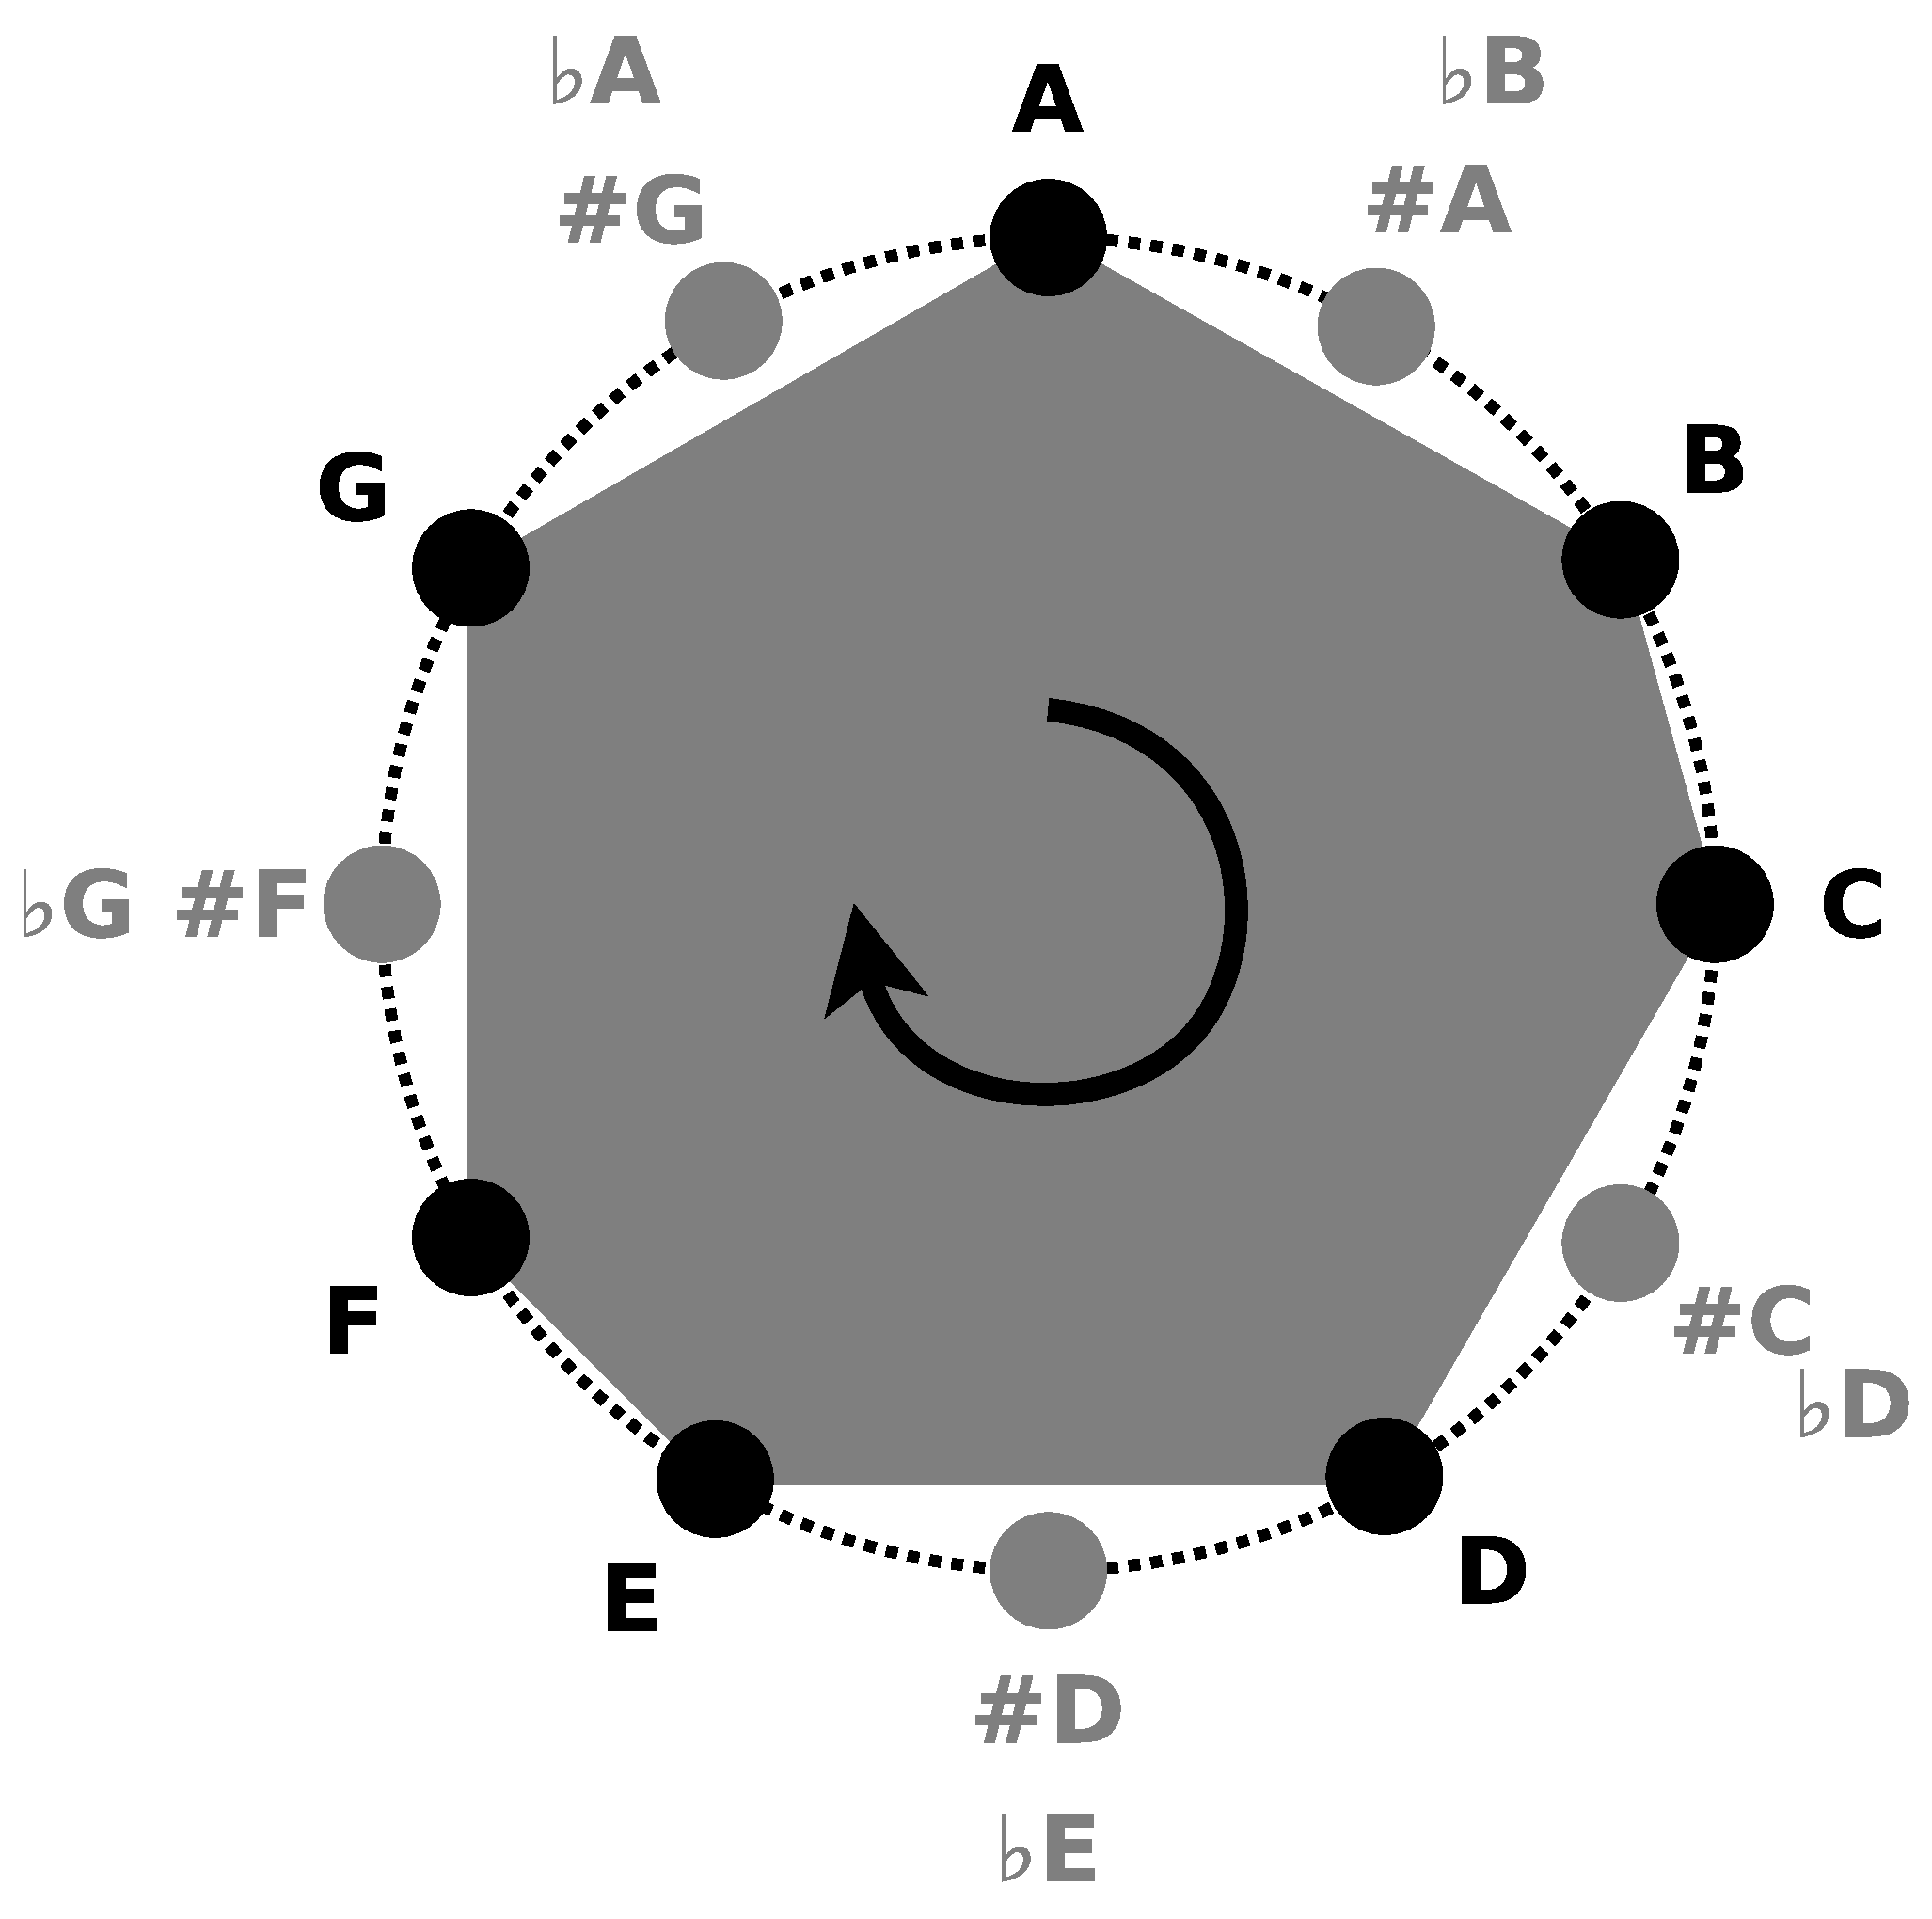
\includegraphics[width=0.65\textwidth]{chapters/cap-musica-basica/circulonotas.eps}
        \caption{Representação cíclica das distancias das notas musicais.}
        \label{fig:circulonotas}
    \end{figure}

Adicionalmente, na Figura \ref{fig:circulonotas}, 
está representada a escala diatônica com uma figura geométrica de 6 lados, 
colorido em cinza; e a escala cromática está representada com um circulo de linha pontuada.


     
%%%%%%%%%%%%%%%%%%%%%%%%%%%%%%%%%%%%%%%%%%%%%%%%%%%%%%%%%%%%%%%%%%%%%%%%%%%%%%%%
\section{\textcolor{blue}{Tipos de pauta}}
\label{sec:tipospauta}

%%%%%%%%%%%%%%%%%%%%%%%%%%%%%%%%%%%%%%%%%%%%%%%%%%%%%%%%%%%%%%%%%%%%%%%%%%%%%%%%
%%%%%%%%%%%%%%%%%%%%%%%%%%%%%%%%%%%%%%%%%%%%%%%%%%%%%%%%%%%%%%%%%%%%%%%%%%%%%%%%
\subsection{Pauta ou Pentagrama}\index{Pauta}
\label{sec:pauta}
A pauta está representada por 5 linhas paralelas e horizontais, 
as figuras musicais podem ocupar as linhas ou um lugar médio, entre elas.
Adicionalmente, lugares fora da pauta podem ser usados; 
para este proposito, linhas adicionais e parcialmente desenhadas, serão colocadas \cite[pp. 10]{cardoso1973curso}
como é mostrado na Figura \ref{fig:abc-pauta5}.
\begin{figure}[H]
\centering
\begin{abc}[name=abc-pauta5]
% abcm2ps pauta5.abc  -O pauta5.ps
% ps2epsi pauta5.ps pauta5.eps
%
X: 1 % start of header
K: none stafflines=5 %K: C %% Escala de C mayor %
M: none % M: 2/4
%T: Contratempo num compasso binário
V:1 clef=none stem=up name="Pauta"   sname="Pauta"
%
[V:1] C8 D8 E8 F8 G8 A8 B8 C'8 D'8 E'8 F'8 G'8 A'8
\end{abc}
\caption{Pauta com 5 linhas e figuras musicais mostrando algumas posições usáveis.}
\label{fig:abc-pauta5}
\end{figure}
A ordem de leitura das figuras musicais na pauta é de esquerda a direita,
e indica o avanço  do tempo;
as posições das linhas indicam um ordem crescente na altura do som que representam as figuras,
contando desde a linha inferior ate a superior. Nesse sentido, 
uma pauta é semelhante a um espectrograma, onde o eixo X representa o tempo,
o eixo Y representa a frequência, e a figuras colocadas em distintas posições do plano XY, descrevem
o comportamento do sonido nesses dois âmbitos. Assim, a Figura \ref{fig:abc-pauta5}
representa um conjunto de 13 sonidos, cada um com a mesma duração; 
porem, executado com diferentes alturas e em ordem crescente, 
desde um sonido grave ate um sonido mais agudo.
\begin{remark}
As linhas da pauta se contam de abaixo para acima.
As figuras musicais, se leem de esquerda direita, para que corresponda com o sentido do avanço do tempo.
\end{remark}


Por outro lado, se as figuras musicais podem ocupar varias posições entre as linhas da pauta,
pois estos lugares representam alturas diferentes do som; então, 
os silêncios não precisam desta característica,
pelo qual os símbolos que representam os silêncios tem uma posição fixa na pauta,
como pode ser visto na Figura \ref{fig:abc-pautasilencio}.
\begin{figure}[h]
\centering
\begin{abc}[name=abc-pautasilencio]
% abcm2ps pautasilencio.abc  -O pautasilencio.ps
% ps2epsi pautasilencio.ps pautasilencio.eps
%
X: 1 % start of header
K: none stafflines=5 %K: C %% Escala de C mayor %
M: none % M: 2/4
%T: Contratempo num compasso binário
V:1 clef=none name="Pauta"   sname="Pauta"
%
[V:1] z8 z4 z2 z1 z/2 z/4 G8 A4 B2 C'1 D'/2 E'/4 
\end{abc}
\caption{Pauta com 5 linhas e silêncios musicais mostrando algumas posições usáveis.}
\label{fig:abc-pautasilencio}
\end{figure}

O ponto mais interessante, é ver a diferencia do uso  da pausa de mínima e da pausa de semibreve,
dado que estes dois tipos de pausa usam o mesmo símbolo, porem em distintas posições.
Na Figura \ref{fig:abc-pautasilencio} a pausa de semibreve, 
está colocada em primeiro lugar desde a esquerda da pauta,
e o símbolo está desenhado unido a parte baixa de uma linha da pauta.
Por outro lado, a pausa de mínima está desenhada no segundo lugar da pauta,
contando desde a esquerda, e se desenha unida à parte de acima de uma linha da pauta.
Estos dois simbolo podem estar desenhados em duas linhas diferentes, 
como no exemplo da Figura \ref{fig:abc-pautasilencio}, ou na mesma linha.

\subsubsection{As claves na pauta}
\label{subsubsec:clavespauta}
A clave, como símbolo, 
se coloca ao inicio da pauta, 
e serve para indicar as alturas das notas na pauta \cite[pp. 179]{apel1969harvard} \cite[pp. 10]{cardoso1973curso}.
Existem 3 tipos de claves\footnote{E varias posições para estas, porem aqui veremos as mas basicas.} que podem ser usadas na pauta, 
assim temos: 
\begin{description}
\item [Clave sol:] Representada pelo símbolo 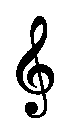
\includegraphics[height=14pt]{chapters/cap-musica-basica/G-clef.eps}. 
A posição donde esta clave se assine indica o lugar onde se localiza uma nota sol.
\begin{example}
Na Figura \ref{fig:abc-clavesol} podemos ver à clave de sol assinada sobre a segunda linha da pauta,
indicando que esta linha representa a nota sol.
\end{example} 
\item [Clave de fá:] Representada pelo símbolo 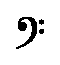
\includegraphics[height=10pt]{chapters/cap-musica-basica/FClef.eps}. 
A posição donde essa clave se assine indica o lugar onde se localiza uma nota fá.
\begin{example}
Na Figura \ref{fig:abc-clavefa} podemos ver à clave de fá assinada sobre a quarta linha da pauta,
indicando que essa linha representa a nota fá.
\end{example} 
\item [Clave de dó:] Representada pelo símbolo 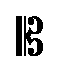
\includegraphics[height=10pt]{chapters/cap-musica-basica/CClef.eps}.
A posição donde esta clave se assine indica o lugar onde se localiza uma nota dó.
\begin{example}
Na Figura \ref{fig:abc-clavedo} podemos ver à clave de dó assinada sobre a terceira linha da pauta,
indicando que essa linha representa a nota dó.
\end{example} 
\end{description}
%%%
\begin{figure}[h]
    \centering
\begin{subfigure}[c]{0.25\textwidth}
\begin{abc}[name=abc-clavesol]
% abcm2ps clavesol.abc  -O clavesol.ps
% ps2epsi clavesol.ps clavesol.eps
%
X: 1 % start of header
K: C stafflines=5 %K: C %% Escala de C mayor %
M: none % M: 2/4
%T: Contratempo num compasso binário
V:1 clef=treble %name="Pauta com clave de sol"   sname="Pauta com clave de sol"
%
[V:1] G8
\end{abc}
\caption{Clave de sol com uma semibreve colocada em sol.}
\label{fig:abc-clavesol}
\end{subfigure}
~ %
\begin{subfigure}[c]{0.25\textwidth}
\begin{abc}[name=abc-clavefa]
% abcm2ps clavesfa.abc  -O clavefa.ps
% ps2epsi clavefa.ps clavefa.eps
%
X: 1 % start of header
K: C stafflines=5 %K: C %% Escala de C mayor %
M: none % M: 2/4
%T: Contratempo num compasso binário
V:1 clef=bass %name="Pauta com clave de fá"   sname="Pauta com clave de fá"
%
[V:1] F,8  
\end{abc}
\caption{Clave de fá com uma semibreve colocada em fá.}
\label{fig:abc-clavefa}
\end{subfigure}
~ %
\begin{subfigure}[c]{0.25\textwidth}
\begin{abc}[name=abc-clavedo]
% abcm2ps clavesfa.abc  -O clavedo.ps
% ps2epsi clavedo.ps clavedo.eps
%
X: 1 % start of header
K: C stafflines=5 %K: C %% Escala de C mayor %
M: none % M: 2/4
%T: Contratempo num compasso binário
V:1 clef=C %name="Pauta com clave de fá"   sname="Pauta com clave de fá"
%
[V:1] C8 
\end{abc}
\caption{Clave de dó com uma semibreve colocada em dó.}
\label{fig:abc-clavedo}
\end{subfigure}
    \caption{Tipos de claves}\label{fig:allclaves}
\end{figure}



\subsubsection{As claves e a escala diatonica}
Conhecida as definições das claves, e da \hyperref[sec:pos:Diatonica]{\textbf{escala diatônica}}, 
podemos misturar estes dois conceitos para conhecer a posição de todas as notas na pauta
\cite[pp. 10]{cardoso1973curso} \cite[pp. 14]{medteoria}.

Por exemplo, as pautas desenhadas na Figura \ref{fig:allnotesclaves} 
contem duas duas oitavas cada uma, centradas em dó, e com notas escritas usando semibreves.
\begin{figure}[h]
    \centering
\begin{abc}[name=abc-clavenotessol]
% abcm2ps clavenotessol.abc  -O clavenotessol.ps
% ps2epsi clavenotessol.ps clavenotessol.eps
%
X: 1 % start of header
K: C stafflines=5 %K: C %% Escala de C mayor %
M: none % M: 2/4
%T: Contratempo num compasso binário
V:1 clef=treble %name="Pauta com clave de sol"   sname="Pauta com clave de sol"
%
[V:1] "dó"C,8 "ré"D,8 "mi"E,8 "fá"F,8  "sol"G,8 "lá"A,8 "si"B,8 "dó"C8 "ré"D8 "mi"E8 "fá"F8  "sol"G8 "lá"A8 "si"B8 "dó"C'8 
\end{abc}

\begin{abc}[name=abc-clavenotesfa]
% abcm2ps clavenotesfa.abc  -O clavenotesfa.ps
% ps2epsi clavenotesfa.ps clavenotesfa.eps
%
X: 1 % start of header
K: C stafflines=5 %K: C %% Escala de C mayor %
M: none % M: 2/4
%T: Contratempo num compasso binário
V:1 clef=bass %name="Pauta com clave de fá"   sname="Pauta com clave de fá"
%
[V:1] C,8 D,8 E,8 F,8 G,8 A,8 B,8 C8 D8 E8 F8 G8 A8 B8 C'8 
\end{abc}

\begin{abc}[name=abc-clavenotesdo]
% abcm2ps clavenotesfa.abc  -O clavenotesdo.ps
% ps2epsi clavenotesdo.ps clavenotesdo.eps
%
X: 1 % start of header
K: C stafflines=5 %K: C %% Escala de C mayor %
M: none % M: 2/4
%T: Contratempo num compasso binário
V:1 clef=C %name="Pauta com clave de fá"   sname="Pauta com clave de fá"
%
[V:1] C,8 D,8 E,8 F,8 G,8 A,8 B,8 C8 D8 E8 F8 G8 A8 B8 C'8 
\end{abc}
    \caption{Tipos de claves}\label{fig:allnotesclaves}
\end{figure}
Na pauta com clave de sol, 
se distingue como as notas da oitava mais alta estão bem posicionadas na pauta;
porem, as notas da oitava inferior precisam linhas adicionais para serem representadas,
o que dificultará ou não deixará muito elegante a leitura dos elementos na pauta.
Podemos ver um caso similar, pero ao contrario, com a pauta que usa uma clave de fá;
nela, as notas da primeira oitava estão comodamente representadas dentro da pauta;
porem, as da oitava superior precisam linhas adicionais.
Finalmente, a notas escritas usando a clave de dó, estão bem centradas,
para notas com alturas intermédias e só fica fora da pauta as duas notas mais aguda e as duas mais graves.

A primeira vista poderia parecer mais vantajosa a clave de do, 
porem isto acontece só porque a nota central que queremos representar é um dó,
teríamos uma vantagem similar na clave de sol, se usaremos uma nota central em si,
ou a vantagem a teríamos na clave de fá, se usaremos uma nota central em ré. 
Na prática, escolher entre
uma clave u outra dependerá da melodia que queiramos encaixar na pauta.
Porem existe uma combinação muito usada na musica para piano, 
que é usar uma clave de sol pra descrever as melodias a serem tocadas pela mão direita,
e usar uma clave de fá, para as que serão tocadas pela mão esquerda; 
isto é conveniente devido a que se olhamos o dó central nessas claves, 
na Figura \ref{fig:allnotesclaves}, 
poderemos observar que esta nota se sai das linhas da pauta, 
justo para entrar nas linhas da pauta da outra mão.

%%%%%%%%%%%%%%%%%%%%%%%%%%%%%%%%%%%%%%%%%%%%%%%%%%%%%%%%%%%%%%%%%%%%%%%%%%%%%%%%
%%%%%%%%%%%%%%%%%%%%%%%%%%%%%%%%%%%%%%%%%%%%%%%%%%%%%%%%%%%%%%%%%%%%%%%%%%%%%%%%
\subsection{\textcolor{green}{Pauta de percussão}}\index{Pauta!Pauta de Percussão}

Existem varias formas de representar as pautas para percussão, 
estas são diferenciadas do pentagrama, devido a que na percussão, 
na maioria dos casos não se tem controle da \hyperref[sec:pos:Duracion]{\textbf{duração}} do som;
e sim se tem, do momento em que este será executado. Em outros casos,
pode estar desabilitada a possibilidade de mudar a \hyperref[sec:pos:Altura]{\textbf{altura}} dos sons;
pelo que não se necessitam linhas pra representar estas alturas.
Assim, as pautas de percussão estarão optimizadas, em cada caso, 
para mostrar com simplicidade o ritmo que se deseja interpretar.

\subsubsection{A clave de percussão}
Também chamada \textbf{clave neutral} ou \textbf{clave de ritmos}, 
porque é usada por percussionistas, bateristas, 
ou usada para qualquer instrumento que produz um som que não tem uma altura definida \cite[pp. 51]{harnum2009basic}.
Asim, esta clave indica que a pauta mostra ritmos e modos de tocar um instrumento, 
e não indica as alturas das notas, 
como outras claves mostradas na Seção \ref{subsubsec:clavespauta}.
Podemos achar dois símbolos equivalentes para representar esta clave, 
estes são \includegraphics[height=10pt]{chapters/cap-musica-basica/P1-clef.eps}
e \includegraphics[height=10pt]{chapters/cap-musica-basica/P2-clef.eps}.
Entre os instrumentos que usam esta clave temos:
o tambourine, o triangulo, o pandeiro, etc.
A Figura \ref{fig:allpercusionclaves} mostra algumas formas de usar a clave de percussão,
sendo formas equivalentes, as mostradas na Figura \ref{fig:abc-claveperczero} e a Figura \ref{fig:abc-clavepercuma}.

\begin{figure}[h]
    \centering 
\begin{subfigure}[c]{0.24\textwidth}
\begin{abc}[name=abc-clavepercusion1]
% abcm2ps clavepercusion1.abc  -O clavepercusion1.ps
% ps2epsi clavepercusion1.ps clavepercusion1.eps
%
X: 1 % start of header
K: C stafflines=0 %K: C %% Escala de C mayor %
M: none % M: 2/4
%T: Contratempo num compasso binário
V:1 clef=perc stem=up %name="Pauta com clave de fá"   sname="Pauta com clave de fá"
%
[V:1] B1 B1 B2 B1 B2   
\end{abc}
\caption{Clave de percussão sem linhas, indicando que só existe um modo de tocar o instrumento.}
\label{fig:abc-claveperczero}
\end{subfigure}
~%
\begin{subfigure}[c]{0.24\textwidth}
\begin{abc}[name=abc-clavepercusion2a]
% abcm2ps clavepercusion2a.abc  -O clavepercusion2a.ps
% ps2epsi clavepercusion2a.ps clavepercusion2a.eps
%
X: 1 % start of header
K: C stafflines=1 %K: C %% Escala de C mayor %
M: none % M: 2/4
%T: Contratempo num compasso binário
V:1 clef=perc stem=up %name="Pauta com clave de fá"   sname="Pauta com clave de fá"
%
[V:1] B1 B1 B2 B1 B2   
\end{abc}
\caption{Clave de percussão com uma linha e só um modo de tocar o instrumento.}
\label{fig:abc-clavepercuma}
\end{subfigure}
~%
\begin{subfigure}[c]{0.24\textwidth}
\begin{abc}[name=abc-clavepercusion2]
% abcm2ps clavepercusion2.abc  -O clavepercusion2.ps
% ps2epsi clavepercusion2.ps clavepercusion2.eps
%
X: 1 % start of header
K: C stafflines=1 %K: C %% Escala de C mayor %
M: none % M: 2/4
%T: Contratempo num compasso binário
V:1 clef=perc stem=up %name="Pauta com clave de fá"   sname="Pauta com clave de fá"
%
[V:1] A1 C'1 A2 C'1 A2   
\end{abc}
\caption{Clave de percussão com uma linha e dois modos de tocar o instrumento.}
\label{fig:abc-clavepercum2}
\end{subfigure}
~%
\begin{subfigure}[c]{0.24\textwidth}
\begin{abc}[name=abc-clavepercusion3]
% abcm2ps clavepercusion3.abc  -O clavepercusion3.ps
% ps2epsi clavepercusion3.ps clavepercusion3.eps
%
X: 1 % start of header
K: C stafflines=5 %K: C %% Escala de C mayor %
M: none % M: 2/4
%T: Contratempo num compasso binário
V:1 clef=perc stem=up %name="Pauta com clave de fá"   sname="Pauta com clave de fá"
%
[V:1] A1 B1 G2 C'1 F2   
\end{abc}
\caption{Clave de percussão com cinco linhas e vários modos de tocar o instrumento.}
\label{fig:abc-claveperccinco}
\end{subfigure}
    \caption{Usos da clave de percussão}\label{fig:allpercusionclaves}
\end{figure}

\subsubsection{O sistema de notação monolinear}
Este sistema foi criado pelo baterista suiço, Dr. Fritz Berger, em 1928. 
Ele o chamou ``the monolinear notation system'', 
de modo que seu sistema utilizava uma única linha na pauta, na sua definição,
a parte de acima da linha representava a mão direita (para bateria), e
a parte de abaixo da linha a mão esquerda.
Assim, era mais fácil ler os ritmos, deixando claro que mão devia fazer uma determinada ação
\cite[pp. 148]{beck1995encyclopedia} \cite[pp. 332]{dean2012drum}.
Um exemplo deste sistema pode ser visto na Figura \ref{fig:abc-clavepercum2}.

\subsubsection{The grid notation}


\cite[pp. 289]{gould676behind}

\begin{comment}
\subsubsection{The musical notation of percusion}
Revisar  \cite[pp. 70]{harnum2009basic}

Figura \ref{fig:abc-musicalperc}
\begin{figure}[H]
\centering
\begin{abc}[name=abc-musicalperc]
% abcm2ps musicalperc.abc  -O musicalperc.ps
% ps2epsi musicalperc.ps musicalperc.eps
%
X:1
T:Drum Key
M:
L:1/4
K:C clef=perc
"^Bass"F|"^Snare"c|"^High tom"e|"^Mid tom"d|"^Low tom"B|"^Floor tom"A|
"^Cymbal"^b|"^Crash"^a|"^Hi-hat"^g|"^Ride"^f|"^Hi-hat Pedal"^D|]

\end{abc}
\caption{Figuras e pausas}
\label{fig:abc-musicalperc}
\end{figure}
\end{comment}


        
%%%%%%%%%%%%%%%%%%%%%%%%%%%%%%%%%%%%%%%%%%%%%%%%%%%%%%%%%%%%%%%%%%%%%%%%%%%%%%%%
\section{\textcolor{green}{Compasso}}\index{Compasso}
\label{sec:compaso}

\begin{description}
\item[Compasso:] O dicionário de Harvard de música \cite[pp. 513]{apel1969harvard} define compasso (``measure'' em inglês)
como um grupo de tempos, batimentos ou pulsos (unidade do tempo musical),
onde o primeiro destes normalmente é acentuado. 
Este número de tempos no compasso pode ser, dois, trés, quatro, ou ocasionalmente 5 ou mais. 
Sendo estos compassos separados por barras verticais e as notas do compasso esquematizados baixo uma métrica.
\begin{example}
Figura \ref{fig:abc-exemplocompasso1}
\end{example}
 
\item[Métrica:] Sobre a métrica  (``meter'' em inglês) o dicionario \cite[pp. 523]{apel1969harvard} explica que é
um padrão de unidades temporais fixas, chamados batimentos, 
pelo qual um período de tempo de uma peça musical ou uma seção dela é medida. 
Agrega tambem que a métrica é indicado geralmente por uma fração, como por exemplo:
${2}/{2}$ , ${3}/{4}$ , ${4}/{4}$, etc. Em português esta fração é chamada de formula do compasso. 
\begin{example}
Figura \ref{fig:abc-exemplocompasso1}
\end{example}
\end{description}

O numerador, da formula do compasso, indica o número de pulsações (tempos) que compõem cada compasso.
Por outro lado o denominador nos informa al longitude temporal de cada um dos tempos do compasso.

\begin{figure}[h]
\centering
\begin{abc}[name=abc-exemplocompasso1]
% abcm2ps exemplocompasso1.abc  -O exemplocompasso1.ps
% ps2epsi exemplocompasso1.ps exemplocompasso1.eps
%
X: 1 % start of header
K: none stafflines=0 %K: C %% Escala de C mayor %
M: 2/4
%T: Contratempo num compasso binário
V:1 clef=perc stem=up name="Ritmo 1"   sname="Ritmo 1"
%
[V:1] | B2 B1 B1| B2 B1 B1 | B2 B1 B1 | B2 z2  |
%       
\end{abc}
\caption{Figuras e pausas}
\label{fig:abc-exemplocompasso1}
\end{figure}



A Tabela \ref{tab:abc-noteslength} exemplifica o significado do denominador da formula do compasso; 
\begin{table}[h]
\centering
\begin{tabular}{|c|c|c|c|}
\hline
denominador & Figura  & Duração & Nome\\ \hline
\hline
$1$   & \fullnote    & $S$   & Semibreve \\ \hline
$2$ & \halfnote    & $S/2$ & Mínima \\ \hline
$4$ & \quarternote & $S/4$ & Semínima \\ \hline
$8$ & \eighthnote  & $S/8$ & Colcheia \\ \hline
\end{tabular}
\caption{Duração e símbolos de algumas figuras musicais}
\label{tab:abc-noteslength}
\end{table}
onde a primeira coluna mostra o denominador da formula,
a segunda coluna mostra as figuras musicais que representam cada um dos tempos do compasso, e 
a terceira e quarta coluna, indicam a duração em segundos e o nome da figura musical.

podemos achar equivalências aos exemplos da formula do compasso dados
anteriormente; onde os compassos com formula $\mathbf{2}/2$ tem cada um, uma duração de $\mathbf{2}$\halfnote ~(duas mínimas),  
compassos com formula $\mathbf{3}/4$ tem uma duração de $\mathbf{3}$\quarternote ~(trés semínimas) 
e $\mathbf{4}/4$ uma duração de $\mathbf{4}$\quarternote ~(quatro semínimas). É importante
ressaltar que a duração em tempo das figuras musicais é relativa, como pode ser visto
na terceira coluna da Tabela \ref{tab:abc-noteslength}, onde as durações estão em função
da duração $S$ da semibreve. 


Se classificamos os compassos por sua métrica, os três tipos mais conhecidos 
são os compassos binários, ternários, quaternários \cite[pp. 27]{adolfo2002musica}.

\subsection{\textcolor{green}{Compasso binário}}\index{Compasso!Compasso Binário} Ou compasso binário simples,
é uma estrutura rítmica que se carateriza por ter compassos com uma  duração de dois tempos,
sendo o primeiro tempo forte (acentuado), e o segundo de tempo fraco (não acentuado)
\cite[pp. 41]{grabner2001teoria} \cite[pp. 66]{adolfo2002musica}\cite[pp. 28]{alves2004teoria}. 
Os compassos binários (simples) tem uma formula de compasso na forma $2/B$,
onde $B$ pode ser $2$, $4$, $8$, etc. 
A Figura \ref{compasso:binario}, representa um exemplo de compasso binário simples, 
com formula de compasso $2/2 \equiv 2$\halfnote, 
e tempos com uma duração de $S/2$ (uma \halfnote), 
sendo que o primeiro compasso contem $2$\halfnote~e o segundo contem $4$\quarternote.
Na Figura \ref{compasso:binario} a sigla ``N.A.'' significa ``Não acentuado'', pelo que é fácil perceber
que em qualquer caso, só a nota que é executada no tempo 1 é acentuada.
\begin{figure}[H]
\centering
\begin{abc}[name=abc-compasso1]
X: 1 % start of header
K: C % scale: C major
M: 2/2 %meter - compasso
"Primeiro compasso" G4 F4 |"Segundo compasso" G2 D2 F2 D2  |
w: Acentuado N.A. Acentuado N.A. N.A. N.A.
\end{abc}
\caption{Exemplo de compasso binário (simples)}
\label{compasso:binario}
\end{figure}

Se falamos de forma mais geral, 
podemos ter dois tipos de compassos binários: os simples e os compostos.
Assim, 
para achar a formula de um compasso composto, correspondente a um compasso simples (usando quialteras de três)
usamos a seguinte operação \cite[pp. 74]{alves2004teoria}, 
\begin{equation}\label{eq:comcomposto}
Compasso~simples\times\frac{3}{2}=Compasso~composto.
\end{equation}
De modo que obtemos compassos binários compostos com as seguintes formulas de compasso: 
$6/4$, $6/8$, $6/16$, etc.
A diferencia do visto nos compassos binários simples, os compassos binários compostos tem 
um pulso forte (Acentuado) no tempo 1 e um pulso semiforte (Acentuado porem menor) no tempo 4, 
de modo que os tempos 2,3,5 e 6,
são classificados como tempos fracos (Não Acentuados)\cite[pp. 41]{grabner2001teoria}.
A Figura \ref{compasso:binariocomposto}, representa um exemplo de compasso binário composto, 
com formula de compasso $6/4 \equiv 6$\quarternote, 
e tempos com uma duração de $S/4$ (uma \quarternote), 
sendo que o primeiro compasso contem $6$\quarternote~e o segundo contem dois $2$\quarternote~e dois $2$\halfnote.
Da Figura \ref{compasso:binariocomposto} é fácil perceber
que em qualquer caso, só são acentuados as nota que são executadas no tempo 1 e 4; 
aclarando que as notas executadas no tempo 4 tem uma acentuação menor que as executadas no tempo 1.
\begin{figure}[H]
\centering
\begin{abc}[name=abc-compasso1c]
X: 1 % start of header
K: C % scale: C major
M: 6/4 %meter - compasso
"Primeiro compasso" G2 D2 D2 F2 D2 D2 |"Segundo compasso" G2 D4 F2 D4  |
w: Acentuado N.A. N.A. Acentuado N.A N.A. Acentuado N.A. Acentuado N.A. 
\end{abc}
\caption{Exemplo de compasso binário composto}
\label{compasso:binariocomposto}
\end{figure}

Alguns autores consideram aos compassos quaternários (ex: 4/4, 4/8) como um caso de compasso binário,
chamando eles de compasso binário duplo \cite[pp. 41]{grabner2001teoria}.




\subsection{\textcolor{green}{Compasso ternário}}\index{Compasso!Compasso Ternário} Ou compasso ternário simples,
é uma estrutura rítmica que se carateriza por ter compassos com trés tempos,
sendo o primeiro pulso forte (acentuado) e os outros dois fracos (não acentuados) 
\cite[pp. 67]{adolfo2002musica}\cite[pp. 30]{alves2004teoria}. 
Os compassos ternários (simples) tem uma formula de compasso da forma $3/B$, 
onde $B$ pode ser $2$, $4$, $8$, etc.
Por exemplo temos, as formulas de compassos ternários simples: $3/2$, $3/4$, $3/8$,  etc.

A Figura \ref{compasso:ternario}, representa um exemplo de compasso ternário (simples), com 
formula de compasso $3/4 \equiv 3$\quarternote, 
onde os tempos tem uma duração de $S/4$, o primeiro compasso contem $3$\quarternote~e
o segundo contem $6$\eighthnote.
Na Figura \ref{compasso:ternario}  é fácil perceber
que em ambos compassos, só a nota que é executada no tempo 1 é acentuada.
\begin{figure}[H]
\centering
\begin{abc}[name=abc-compasso2]
X: 1 % start of header
K: C % scale: C major
M: 3/4 %meter - compasso
"Primeiro compasso" G2 F2 F2 |"Segundo compasso" G1 F1 E1 D1 D1  D1  |
w: Acentuado N.A. N.A. Acentuado N.A N.A.  N.A. N.A. N.A. 
\end{abc}
\caption{Exemplo de compasso ternário}
\label{compasso:ternario}
\end{figure}


São chamados de compassos ternários compostos,  
quando estes tem uma formula de compasso como: $9/4$, $9/8$ e $9/16$.
Para gerar estes compassos compostos a partir de suas versões simples,
se segue a mesma operação descrita na Equação \ref{eq:comcomposto}.


\subsection{\textcolor{green}{Compasso quaternário}}\index{Compasso!Compasso Quaternário} Ou compasso quaternário simples,
é uma estrutura rítmica que se carateriza por ter compassos com quatro tempos,
sendo o primeiro pulso forte (acentuado), o segundo fraco (não acentuado), 
o terceiro semiforte (acentuado porem menor) e o último fraco (não acentuado) 
\cite[pp. 67]{adolfo2002musica}\cite[pp. 32]{alves2004teoria}. 
Os compassos quaternários (simples) tem uma formula de compasso da forma $4/B$, 
onde $B$ pode ser $2$, $4$, $8$, etc.
Por exemplo temos, as formulas de compassos ternários simples: $4/2$, $4/4$, $4/8$,  etc.

A Figura \ref{compasso:quaternario}, representa um exemplo de compassos quaternário, com 
formula de compasso $4/4 \equiv 4$\quarternote, 
onde cada tempo tem uma duração de $S/4$, o primeiro compasso contem $4$\quarternote~e
o segundo contem $8$\eighthnote.
Na Figura \ref{compasso:ternario}  é fácil perceber
que em ambos compassos, só as notas que são executadas no tempo 1 e 3 são acentuadas.
\begin{figure}[H]
\centering
\begin{abc}[name=abc-compasso3]
X: 1 % start of header
K: C % scale: C major
M: 4/4 %meter - compasso
"Primeiro compasso" G2 D2 F2 D2|"Segundo compasso" G1 F1 D1 C1 F1 E1 D1 C1 |
w: Acentuado N.A. Acentuado N.A. Acentuado N.A N.A. N.A. Acentuado N.A. N.A. N.A. 
\end{abc}
\caption{Exemplo de compasso quaternário}
\label{compasso:quaternario}
\end{figure}

São chamados de compassos quaternários compostos,  
quando estes tem uma formula de compasso como: $12/4$, $12/8$ e $12/16$.
Para gerar estes compassos compostos a partir de suas versões simples,
se segue a mesma operação descrita na Equação \ref{eq:comcomposto}.
 

%%%%%%%%%%%%%%%%%%%%%%%%%%%%%%%%%%%%%%%%%%%%%%%%%%%%%%%%%%%%%%%%%%%%%%%%%%%%%%%%

\section{Ligadura}
\index{Música!Ligadura}
\label{sec:ligadura}

A ligadura é uma linha curva que se coloca sobre duas ou mais notas da mesma altura, 
indicando que somente a primeira é articulada, 
e esta tem uma duração equivalente a soma de todas as notas ligadas \cite[pp. 35]{cardoso1973curso}.

\begin{example}
A Figura \ref{fig:total-ligadura} descreve 3 casos de uso de ligadura.
\begin{itemize}
\item Na Figura \ref{fig:abc-ligadura1} pode-se ver que, no primeiro compasso, 
tem-se uma ligadura entre a primeira e a segunda figura musical; 
no segundo compasso tem-se uma representação equivalente ao primeiro compasso; 
porém, usando ponto de aumento.
\item Na Figura \ref{fig:abc-ligadura2} pode-se ver que, no primeiro compasso, 
tem-se ligaduras entre as três primeiras figuras musicais; 
no segundo compasso tem-se uma representação equivalente ao primeiro compasso; 
porém, usando dois pontos de aumento.
\item Na Figura \ref{fig:abc-ligadura3} tem-se um exemplo de uso de ligadura entre figuras musicais de diferentes compassos,
de modo que a duração da última nota, do primeiro compasso, se prolonga até o segundo compasso.
\end{itemize}
\end{example}


\begin{figure}[!ht]
    \centering
    \begin{subfigure}[b]{0.6\textwidth}
\begin{abc}[name=abc-ligadura1]
X: 1 % start of header
K: C %% Escala de C mayor %
M: 2/4
%T: Contratempo num compasso binário
V:1 clef=G  %name="Ritmo 1"   sname="Ritmo 1"
%
[V:1] | (B2 B1) C1 | B3 C1   |    
\end{abc}
\vspace{-10pt}
\caption{Uso de ligaduras entre duas notas}
\label{fig:abc-ligadura1}
    \end{subfigure}
    ~%add desired spacing between images, e. g. ~, \quad, \qquad, \hfill etc. 
      %(or a blank line to force the subfigure onto a new line)
    \begin{subfigure}[b]{0.6\textwidth}
\begin{abc}[name=abc-ligadura2]
X: 1 % start of header
K: C %% Escala de C mayor %
M: 2/4
%T: Contratempo num compasso binário
V:1 clef=G  %name="Ritmo 1"   sname="Ritmo 1"
%
[V:1] | (A2 (A1) A1/2) C1/2 | A7/2 C1/2  |
\end{abc}
\vspace{-10pt}
\caption{Uso de ligaduras entre três notas.}
\label{fig:abc-ligadura2}
    \end{subfigure}
    ~%add desired spacing between images, e. g. ~, \quad, \qquad, \hfill etc. 
      %(or a blank line to force the subfigure onto a new line)
    \begin{subfigure}[b]{0.6\textwidth}
\begin{abc}[name=abc-ligadura3]
X: 1 % start of header
K: C %% Escala de C mayor %
M: 2/4
%T: Contratempo num compasso binário
V:1 clef=G  %name="Ritmo 1"   sname="Ritmo 1"
%
[V:1] | B3  (G1 | G2) B2  |
\end{abc}
\vspace{-10pt}
\caption{Uso de ligaduras em notas de compassos distintos.}
\label{fig:abc-ligadura3}
    \end{subfigure}
    \caption{Distintos usos da ligadura.}\label{fig:total-ligadura}
\end{figure}


%%%%%%%%%%%%%%%%%%%%%%%%%%%%%%%%%%%%%%%%%%%%%%%%%%%%%%%%%%%%%%%%%%%%%%%%%%%%%%%%
\section{Tempo}
\index{Tempo}
\label{sec:Tempo}

Como já foi sugerido na Seção \ref{sec:compaso}, é chamado de "tempo" 
à pulsação básica que é usada como unidade de medida das composições musicais.
Os tempos ao ser agrupados em compassos podem formar diferentes estruturas como por exemplo: 
\hyperref[subsec:compassobinario]{\textbf{compassos binários}}, \hyperref[subsec:compassoternario]{\textbf{ternários}} e \hyperref[subsec:compassoquaternario]{\textbf{quaternários}}; que tem uma duração de 2 tempos, 
3 tempos e 4 tempos, respetivamente. 

\begin{notation}[] Para o melhor entendimento das seguintes seções usaremos algumas notações.
\begin{itemize}
\item A variável $T$ será usada para designar à duração em segundos de cada tempo,
sendo que o valor de $T$ variará dependendo da formula do compasso usada.

\item As subdivisões dos tempos serão designadas com as seguintes variáveis:
\begin{itemize}
\item ``FF'' indica que é a parte forte de um tempo forte,
\item ``Ff'' indica que é a parte fraca de um tempo forte,
\item ``fF'' indica que é a parte forte de um tempo fraco,
\item ``ff'' indica que é a parte fraca de um tempo fraco.
\end{itemize}
\end{itemize}

\end{notation}

\subsection{Tempos fortes e fracos}
\index{Tempo!Tempo forte}
\index{Tempo!Tempo fraco}

A formula do compasso de uma peça musical ou uma porção dela, 
nos indica quantos tempos e que duração terão estes tempos no compasso; 
porem, além destas informações, 
a formula do compasso também nos indica o \hyperref[def:acentometrico]{\textbf{acento métrico}} \cite[pp. 70]{cardoso1973curso}; 
é dizer quias serão os tempos fortes, semifortes e fracos no compasso.


\begin{description}
\item[O acento métrico] \label{def:acentometrico} é constituído pelas acentuações fortes e fracas dos tempos dos compassos, 
os acentos métricos não precisam ser grafados na pauta \cite[pp. 141]{medteoria}.
\item[O tempo forte (F)] \label{def:tempoforte} sempre será o primeiro tempo de cada compasso. 
Um tempo forte não necessita uma grafia especial que indique que este deve ser articulado
com maior \hyperref[sec:pos:Intensidade]{\textbf{intensidade}}; é dizer, com acentuação.
\item[O tempo semiforte (sF)] \label{def:temposemiforte} acontece em alguns tipos de compasso, 
como nos compassos quaternários. 
Um tempo semiforte terá uma acentuação menor à do tempo forte, porem maior à de um tempo fraco. 
Este tempo não necessita uma grafia especial que indique que deve ser articulado
com \hyperref[sec:pos:Intensidade]{\textbf{intensidade}}.
\item[O tempo fraco (f)] \label{def:tempofraco} corresponde a todos os tempos que não sejam né fortes, né semifortes,
de modo que estes tempos não tem acentuação. 
\end{description}~

Uma versão mais simplificada das informações dadas anteriormente, 
pode ser vista na seguinte equação que mostra a relação de \hyperref[sec:pos:Intensidade]{\textbf{intensidades}}:
\begin{equation}
f ~<~ sF ~<~ F.
\end{equation}

Porem, 
se utilizamos as subdivisões de tempos, 
a relação de \hyperref[sec:pos:Intensidade]{\textbf{intensidades}} pode ser expressada mediante a seguinte equação:
\begin{equation}
\{fF=ff\} ~<~  \{f = fF\} ~<~ sF ~<~ \{F = FF\} 
\end{equation}

\begin{remark}
A regularidade na distribuição das acentuações nos tempos, 
só mudará quando se especifiquem  explicitamente dinâmicas sobre as figuras musicais,
de modo que estas dinâmicas modificam as acentuações,
porem não trocam o nome dos tempos, sendo estes sempre chamados de tempos fortes, semifortes e fracos. 
\end{remark}


\begin{example}
Na Figura \ref{fig:abc-tempo1} podemos ver 2 compassos com a mesma métrica, 
tendo eles uma formula de compasso 2/2; é dizer, 
cada compasso tem dois tempos, como uma duração de uma mínima (\halfnote) para cada tempo.
\begin{itemize}
\item O primeiro compasso é preenchido com duas notas que usam figuras musicais que duram um tempo cada um;
de modo que 
a primeira nota será executada no tempo forte, 
possuindo esta nota um \hyperref[def:acentoprincipal]{\textbf{acento  principal}}, e 
a segunda nota é executada no tempo fraco e não leva acento; 
é dizer tem um menor \hyperref[sec:pos:Intensidade]{\textbf{intensidade}} que a nota do primeiro tempo.
\item No segundo compasso, este é preenchido com 4 notas que usam figuras musicais que duram 1/2 tempo cada uma;
Assim, 
\begin{itemize}
\item a primeira nota será executada em FF (acentuada como F),
\item a segunda  nota será executada em Ff (menos acentuada que f),
\item a terceira nota será executada em fF (acentuada como f), e 
\item a quarta   nota será executada em ff (menos acentuada que f).
\end{itemize}
\end{itemize} 
\end{example}
\begin{figure}[H]
\centering
\begin{abc}[name=abc-tempo1,width=0.6\linewidth]
X: 1 % start of header
K: none stafflines=0 %K: C %% Escala de C mayor %
M: 2/2 %meter - compasso
V:1 clef=perc stem=up name="Ritmo"   sname="Ritmo"
[V:1] | B4 B4 |  B2 B2 B2 B2 |  
w:  T T    T/2 T/2 T/2 T/2 
w:  F f FF Ff fF ff
\end{abc}
\caption{Dois compassos com 2 tempos cada um.}
\label{fig:abc-tempo1}
\end{figure}


\begin{example}
Na Figura \ref{fig:abc-tempo2} podemos ver 2 compassos com a mesma métrica, 
tendo eles uma formula de compasso 4/4; é dizer, 
cada compasso tem quatro tempos, como uma duração de uma semínima (\quarternote) para cada tempo.
\begin{itemize}
\item O primeiro compasso é preenchido com duas notas que usam figuras musicais que duram dois tempos cada um;
de modo que a primeira nota será executada no tempo forte,
possuindo esta nota um \hyperref[def:acentoprincipal]{\textbf{acento  principal}}, 
e o som será sustenido ate completar o seguinte tempo fraco, 
a segunda nota será executada no tempo semiforte,
possuindo esta nota um \hyperref[def:acentosecundario]{\textbf{acento  secundario}},
 e o som será sustenido ate completar o seguinte tempo fraco.
Em ambas figuras não são colocados os símbolos, F e sF, 
pois as notas ocupam mais de um tempo, porem as acentuações são respeitadas.
\item O segundo compasso é preenchido com 4 notas que usam figuras musicais que duram 1 tempo cada uma;
Assim, 
a primeira nota será executada no tempo forte (F),
a segunda  nota será executada no tempo fraco (f),
a terceira nota será executada no tempo semiforte (sF), e 
a quarta   nota será executada no tempo fraco (f).
\end{itemize} 
\end{example}
\begin{figure}[H]
\centering
\begin{abc}[name=abc-tempo2,width=0.6\linewidth]
X: 1 % start of header
K: none stafflines=0 %K: C %% Escala de C mayor %
M: 4/4 %meter - compasso
V:1 clef=perc stem=up name="Ritmo"   sname="Ritmo"
[V:1] | B4  B4 | B2 B2 B2 B2 | 
w:  2T 2T      T T T T 
w:  Acento Acento      F f sF f 
\end{abc}
\caption{Dois compassos com 4 tempos cada um.}
\label{fig:abc-tempo2}
\end{figure} 

\begin{remark}
As pautas mostradas na Figura \ref{fig:abc-tempo1} e na Figura \ref{fig:abc-tempo2},
tem a mesma distribuição de figuras musicais, porem usam formulas do compasso distintas;
Por este pequeno detalhe o som de ambos ritmos será diferente,
pois as acentuações serão diferentes.
Por exemplo, 
na segunda nota do primeiro compasso, na Figura \ref{fig:abc-tempo1}, 
a nota é acentuada como uma f. Porem, 
na  Figura \ref{fig:abc-tempo1}, a nota é acentuada como uma sF, tendo esta ultima maior intensidade.
Existe um caso similar na terça nota do segundo compasso de ambas figuras.

\end{remark}

\subsection{Contagem dos tempos das figuras musicais}
A contagem dos tempos das figuras musicais dentro do compasso, 
acompanha a posição das figuras musicais ou notas dentro do compasso. 
É importante ter em conta a duração das figuras musicais pois a seguinte contagem 
acontece no inicio da seguinte figura musical;
assim, dependendo da duração da figura musical, 
alguns dos tempos do compasso serão contados e outras não \cite[pp. 8]{phillips2002sight}

\begin{example}
A Figura \ref{fig:abc-contagemtempo44} mostra um ritmo que usa 4 compassos quaternários,
com tempos com uma duração de um \quarternote;
assim a contagem dos tempos dentro do compasso vão de 1 ate 4.
Pela irregularidade na duração das figuras musicais alguns tempos não são contados explicitamente.
A contagem pode ser visto na parte superior de cada figura musical.
\end{example}
\begin{figure}[H]
\centering
\begin{abc}[name=abc-contagemtempo1,width=\linewidth]
X: 1 % start of header
K: none stafflines=0 %K: C %% Escala de C mayor %
M: 4/4 %meter - compasso
V:1 clef=perc stem=up name="Ritmo"   sname="Ritmo"
[V:1] | "1"B4  "3"B4 | "1"B8 |  "1"B2 "2"B4 "4"B2 |  "1"B2 z2 "3"B2  z2| 
w:      2T 2T          4T       T 2T T               T T
\end{abc}
\caption{Sequencia rítmica usando um compasso quaternário.}
\label{fig:abc-contagemtempo44}
\end{figure} 



\begin{example}
A Figura \ref{fig:contartempos24}  mostra um ritmo que usa 6 compassos binários,
com tempos com uma duração de um \quarternote;
assim a contagem dos tempos dentro do compasso só pode ser 1 ou 2.
Na parte superior de cada figura musical pode verse a contagem que deve ser feita no ritmo.
\end{example}
\begin{figure}[H]
    \centering
 \begin{abc}[name=abc-contartempos24]
% abcm2ps contartempos24.abc  -O contartempos24.ps
% ps2epsi contartempos24.ps contartempos24.eps
%
X: 1 % start of header
K: none stafflines=0 %K: C %% Escala de C mayor %
M:  2/4
%T: Contratempo num compasso binário
V:1 clef=perc stem=up name="Ritmo"   sname="Ritmo"
%
[V:1] | "1"B2 z2  |"1"B2 "2"B2  | z2 "2"B2  |"1"B4  |"1"B2 "2"B2  |"1"B2 "2"B2  |
w:         T          T  T        T             2T      T T           T T
%       
\end{abc}
\caption{Sequencia rítmica usando um compasso binário.}
\label{fig:contartempos24}
\end{figure}

\begin{comment} 
\begin{example}
A Figura \ref{fig:contartempos34}   mostra um ritmo que usa 4 compassos ternários,
com tempos com uma duração de um \quarternote;
assim a contagem dos tempos dentro do compasso só pode ser 1, 2 ou 3.
Na parte superior de cada figura musical pode verse a contagem que deve ser feita no ritmo.
\end{example}
\begin{figure}[h]
    \centering
 \begin{abc}[name=abc-contartempos34]
% abcm2ps contartempos34.abc  -O contartempos34.ps
% ps2epsi contartempos34.ps contartempos34.eps
%
X: 1 % start of header
K: none stafflines=0 %K: C %% Escala de C mayor %
M:  3/4
%T: Contratempo num compasso binário
V:1 clef=perc stem=up name="Ritmo"   sname="Ritmo"
%
[V:1] | "1"B4 "3"B2 |"1"B2 "2"B2 "3"B2  | z2 "2"B2 "3"B2  |"1"B2 "2"B4  |
%       
\end{abc}
\caption{Sequencia rítmica usando um compasso ternário.}
\label{fig:contartempos34}
\end{figure}
\end{comment} 

%%%%%%%%%%%%%%%%%%%%%%%%%%%%%%%%%%%%%%%%%%%%%%%%%%%%%%%%%%%%%%%%%%%%%%%%%%%%%%%%
\section{\textcolor{green}{Contratempo}}\index{Contratempo}
Um contratempo acontece quando as notas (representadas por figuras musicais na partitura) 
são executadas em tempos fracos do compasso
ou nas partes fracas dos tempos, sendo que estas estão intercaladas por pausas nos tempos
fortes ou partes fortes dos tempos \cite[pp. 16]{mascarenhascurso} 
\cite[pp. 36]{azevedocompor}, neste sentido o contratempo pode ser visto como a 
omissão de notas nos tempos fortes ou nas partes fortes dos tempos \cite[pp. 146]{medteoria}.
Ou ``num sentido mais amplo, o contratempo é a acentuação de um tempo fraco em vez de um tempo forte'' \cite[pp. 147]{medteoria}. 

Assim, a palavra ``contratempo'', referencia a como estão configuradas ou acentuadas 
as notas no compasso. Por exemplo:
A Figura \ref{fig:contratempoa} mostra 
quatro compassos (binários) com formula $2/4$, em cada compasso existem 
contratempos nos tempos fracos ou nas partes fracas dos tempos, sendo que cada tempo
tem uma duração de uma semínima (\quarternote) e cada compasso uma duração 
de uma mínima (\halfnote), ou seja duas semínimas (2\quarternote). 
\begin{itemize}
\item ``F''  indica que é o tempo é forte, 
\item ``f''  indica que é o tempo é fraco,
\item ``FF'' indica que é a parte forte de um tempo forte,
\item ``Ff'' indica que é a parte fraca de um tempo forte,
\item ``fF'' indica que é a parte forte de um tempo fraco,
\item ``ff'' indica que é a parte fraca de um tempo fraco, 
\end{itemize} 

finalmente
a figura musical \ViPa~ indica um silencio da mesma duração que uma semínima (\quarternote)
e a figura musical \AcPa~ indica um silencio da mesma duração que uma colcheia (\eighthnote).
\begin{figure}[H]
\centering
\begin{abc}[name=abc-contratempoa]
X: 1 % start of header
K: C % scale: C major
M:2/4
%T: Contratempo num compasso binário
V:1 clef=treble name="A" sname="A"
[V:1] "F"z2 "f"G2 | "FF"z1 "Ff"G1  "fF"z1 "ff"G1 | "FF"z1 "Ff"G1  "f"G2 |  "F"z2 "fF"z1 "ff"G1  |
w:          T          T/2            T/2             T/2     Tempo                 T/2
\end{abc}
\caption{Contratempos no tempos fracos ou nas partes fracas dos tempos}
\label{fig:abc-contratempoa}
\end{figure}
Na Figura \ref{fig:abc-contratempoa}, existem contratempos em todos os compassos porem estes estão
configurados de distintas formas;
no primeiro compasso acontece um contratempo dado que a única nota é executada 
no tempo fraco do compasso, no segundo compasso acontecem contratempos pois as 
notas são executadas nas partes fracas de cada tempo,
no terceiro compasso acontece um contratempo pela execução de uma nota na parte 
fraca do tempo forte, sendo o resto do tempo preenchido com um silencio, e 
finalmente no quarto compasso acontece um contratempo pela execução de uma nota
na parte fraca do tempo fraco, sendo o resto do compasso preenchido com silêncios.


Por outro lado, 
a Figura \ref{fig:abc-contratempob} mostra um caso similar ao da Figura \ref{fig:abc-contratempoa},
com contratempos expressados como a acentuação de um tempo fraco em vez de um silencio no tempo forte \cite[pp. 147]{medteoria}. 
É usado o símbolo $>$ para indicar esta acentuação na partitura.
\begin{figure}[H]
\centering
\begin{abc}[name=abc-contratempob]
X: 1 % start of header
K: C % scale: C major
M:2/4
%T: Contratempo num compasso binário
V:1 clef=treble name="A" sname="A"
[V:1] "F"G2 "f"+accent+G2 | "FF"G1 "Ff"+accent+G1  "fF"G1 "ff"+accent+G1 | "FF"G1 "Ff"+accent+G1  "f"G2  | "F"G2 "fF"G1  "ff"+accent+G1  | 
w:    T     T                T/2    T/2             T/2    T/2              T/2    T/2             T       T      T/2             T/2  
\end{abc}
\caption{Contratempos pela acentuação dos tempos fracos ou nas partes fracas dos tempos}
\label{fig:abc-contratempob}
\end{figure}

%%%%%%%%%%%%%%%%%%%%%%%%%%%%%%%%%%%%%%%%%%%%%%%%%%%%%%%%%%%%%%%%%%%%%%%%%%%%%%%%
\section{\textcolor{red}{Sincopa}}\index{Sincopa}

%%%%%%%%%%%%%%%%%%%%%%%%%%%%%%%%%%%%%%%%%%%%%%%%%%%%%%%%%%%%%%%%%%%%%%%%%%%%%%%%





